% This is a Beamer template was downloaded from overlead.com , edited and updated to fit ML introduction.
\documentclass{beamer}
\usepackage{graphicx}
\usepackage{media9}

\mode<presentation>{
\usetheme{Dresden}
\setbeamercovered{transparent}
\usecolortheme{lsc}
}

\mode<handout>{
  % tema simples para ser impresso
  \usepackage[bar]{beamerthemetree}
  % Colocando um fundo cinza quando for gerar transparências para serem impressas
  % mais de uma transparência por página
  \beamertemplatesolidbackgroundcolor{black!5}
}

\usepackage{amsmath,amssymb}
\usepackage[brazil]{varioref}
\usepackage[english,brazil]{babel}
\usepackage[utf8]{inputenc}
%\usepackage[latin1]{inputenc}
\usepackage{graphicx}
\usepackage{listings}
\usepackage{url}
\usepackage{colortbl}

\beamertemplatetransparentcovereddynamic

\title[Machine learning]{Machine learning  }
\author[BERRIMI Mohamed]{%
  \textbf{BERRIMI Mohamed}\\
{\small   Master in Data engineering and web technologies \\
 Machine learning enthusiast}}
  \institute[UFAS1]{
 
     University of Ferhat Abbas 1 , Setif \\
     Setifian Scientific Club SeSC\\
 Setifian Developers Group SDG \\ }

% Se comentar a linha abaixo, irá aparecer a data quando foi compilada a apresentação  
\date{22nd May, 2019 }

\pgfdeclareimage[height=0.5cm]{inf}{figs/CienciaDaComputacao.png}

% pode-se colocar o LOGO assim
\logo{\pgfuseimage{inf}}

\AtBeginSection[]{
  \begin{frame}<beamer>
    \frametitle{What is covered in this lecture}
    \tableofcontents[currentsection,currentsubsection]
  \end{frame}
}

\begin{document}

\begin{frame}
\titlepage
\end{frame}

\begin{frame}
\frametitle{What is covered in this lecture}
\tableofcontents
\end{frame}


\section{Introduction }
\frame{
    \frametitle{Introduction}
"People don't know what they are looking for untill you show them" Steve Jobs.
          
 
}
\frame{
	\frametitle{Introduction}
	"people don't know what they are looking for untill you show them" S. Jobs.
	
	It is certain that you have used at least  one  Machine learning method this day
}
\frame{
	\frametitle{Introduction -suite-}
	Google search 
	\center
	\pgfdeclareimage[height=0.9cm]{CDCS}{figs/google.png}
	\pgfuseimage{CDCS}
}

\frame{
	\frametitle{Introduction -suite-}
	Google image search 
	\center
	\pgfdeclareimage[height=4.9cm]{CDCS}{figs/im.jpg}
	\pgfuseimage{CDCS}
}

\frame{

	\frametitle{Introduction -suite-}
 
		Gmail reply recommendation 
	\center

	\pgfdeclareimage[height=4.7cm]{CDCS}{figs/pawel.png}
	\pgfuseimage{CDCS}
}

\frame{
	\frametitle{Introduction -suite-}
	Phones assistants 
	\center
	\pgfdeclareimage[height=05.9cm]{CDCS}{figs/siri.jpg}
	\pgfuseimage{CDCS}
}
\frame{
	\frametitle{Introduction -suite-}
	Youtube Captions 
	\center
	\pgfdeclareimage[height=05cm]{CDCS}{figs/beng.png}
	\pgfuseimage{CDCS}
}


\pgfdeclareimage[height=7cm,width=6cm]{YARNArq}{figs/s1.png}%
\pgfdeclareimage[height=4cm]{HDFSArq}{figs/s.png}%
\frame{
	\frametitle{Introduction - suite -Facebook ML }
	\begin{columns}
		\frametitle{introduction -suite- }
		\column{3cm}
		
		
		\pgfuseimage{YARNArq}
		\begin{tiny}
			
			Covered image [Predicted to be violence or innapropriate]	 
		\end{tiny}
		\column{5cm}
		
		
		\pgfuseimage{HDFSArq}
		\begin{tiny}
			
			(True image )
		\end{tiny}
	\end{columns}
	
}

\pgfdeclareimage[height=6cm]{YARNArq}{figs/fb2.png}%
\pgfdeclareimage[height=3cm]{HDFSArq}{figs/fb3.png}%
\frame{
	\frametitle{Introduction - suite - Facebook ML}
	\begin{columns}
 
	\column{3cm}
 
 
	\pgfuseimage{YARNArq}
	\begin{tiny}
		
	
	Facebook image prediction 
	\end{tiny}
	\column{5cm}
 
 
	\pgfuseimage{HDFSArq}
	\begin{tiny}
		
		(True image )
	\end{tiny}
\end{columns}
 
}

 \frame{
 	\frametitle{HOW ? }
 	
 	\textbf{How the HECK Google and Facebook are doing that ???}
 }

 


\section{Machine learning  }


 
\frame{
 	\frametitle{Definitions }

Learning	is	any	process	by	which	a	system	improves	
performance	from	experience.

}

\frame{
	\frametitle{Definitions }
 
	\center
	\pgfdeclareimage[height=05.9cm]{CDCS}{figs/ml.png}
	\pgfuseimage{CDCS}
}

\logo{\pgfuseimage{inf}}
\frame{
	\frametitle{Definitions.. }
 
 \center
 \pgfdeclareimage[height=05cm]{CDCS}{figs/tom.png}
 \pgfuseimage{CDCS}
}
\section{ML applications}

\frame{
	\frametitle{Where Machine learning  is applied ? }
The use of machine learning is becoming very important and essential in many companies such as Google, Facebook, Apple , Amazon, Netflix .. etc
	
}

\frame{
	\frametitle{Where Machine is applied ? }
	The use of machine learning is becoming very important and essential in many companies such as Google, Facebook, Apple , Amazon, Netflix .. etc\\
	
	Machine learning can also be applied in our life, it can improve many sides of our daily life 	
	
}



\frame{
	\frametitle{ Recommendation systems  }
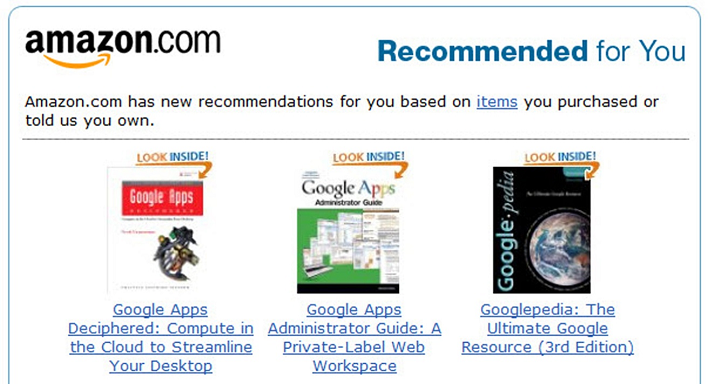
\includegraphics[width=0.6\textwidth]{figs/amazon.png}%
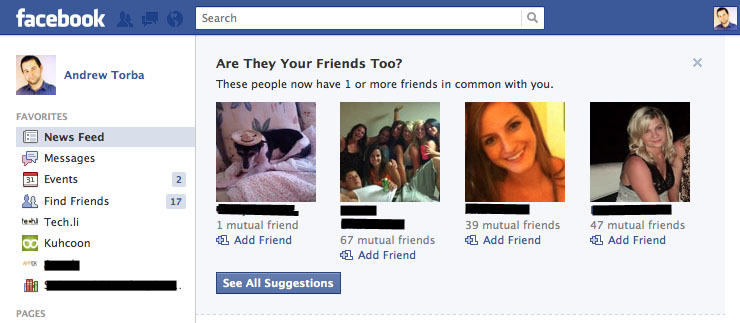
\includegraphics[width=0.4\textwidth]{figs/fb.jpg}
	
}
\frame{
	\frametitle{ Recommendation systems  }
	
\includegraphics[width=1\textwidth]{figs/Netflix.jpg}%

}

\frame{
	\frametitle{ Medical imaging analysis  }
	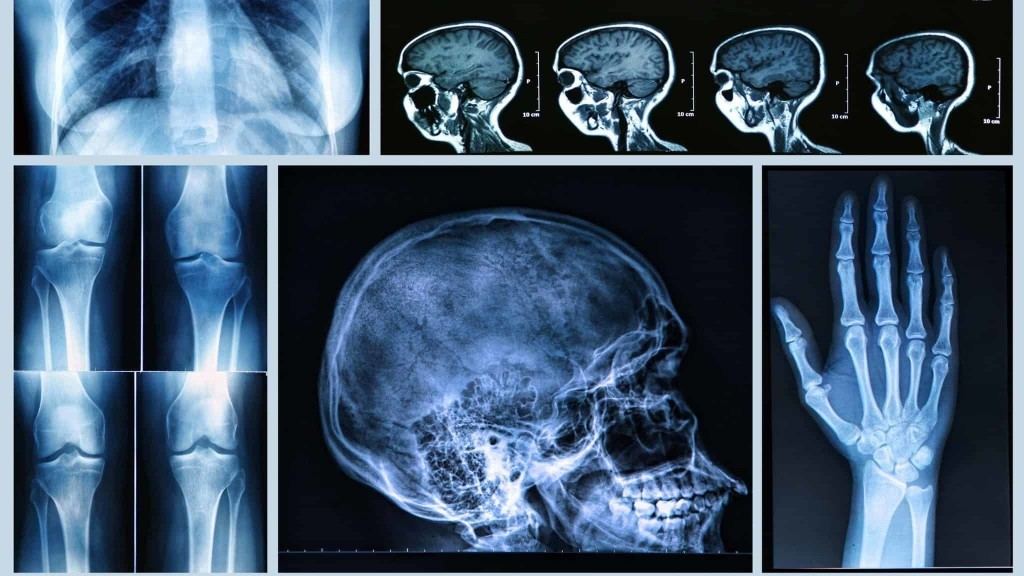
\includegraphics[width=1\textwidth]{figs/m1.jpg}%
	
}

\frame{
	\frametitle{ Medical imaging   }
	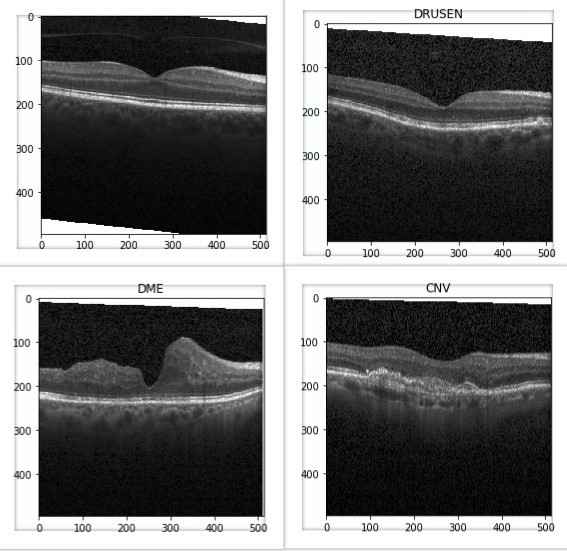
\includegraphics[width=0.6\textwidth]{figs/m1.jpeg}%
	
}
\frame{
	\frametitle{ Machine learning in security   }
	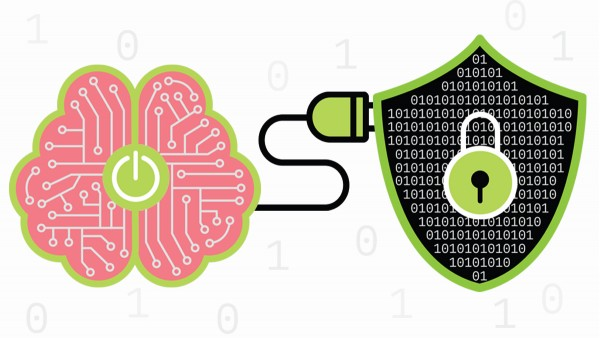
\includegraphics[width=1\textwidth]{figs/sec.jpg}%
	
}
\frame{
	\frametitle{ Self driving cars    }
	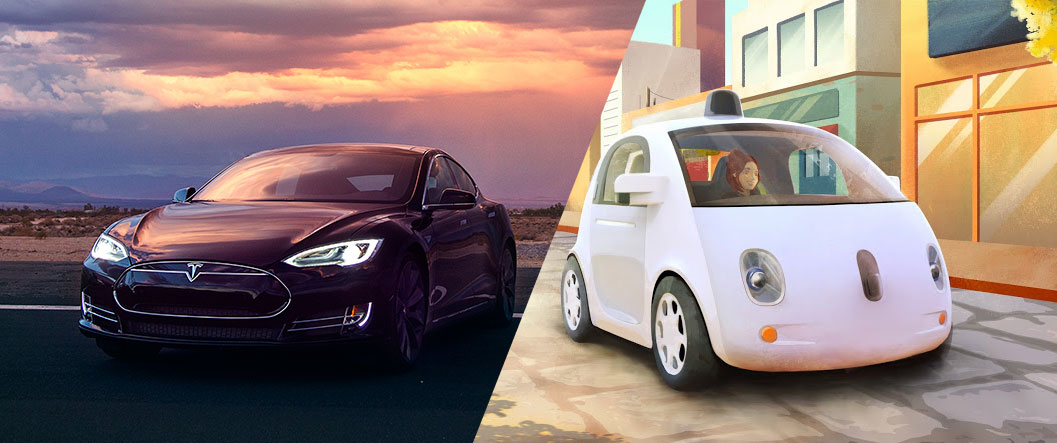
\includegraphics[width=1\textwidth]{figs/tesla.jpg}%
	
}

\frame{

	\frametitle{ Voice recognition   }
 
	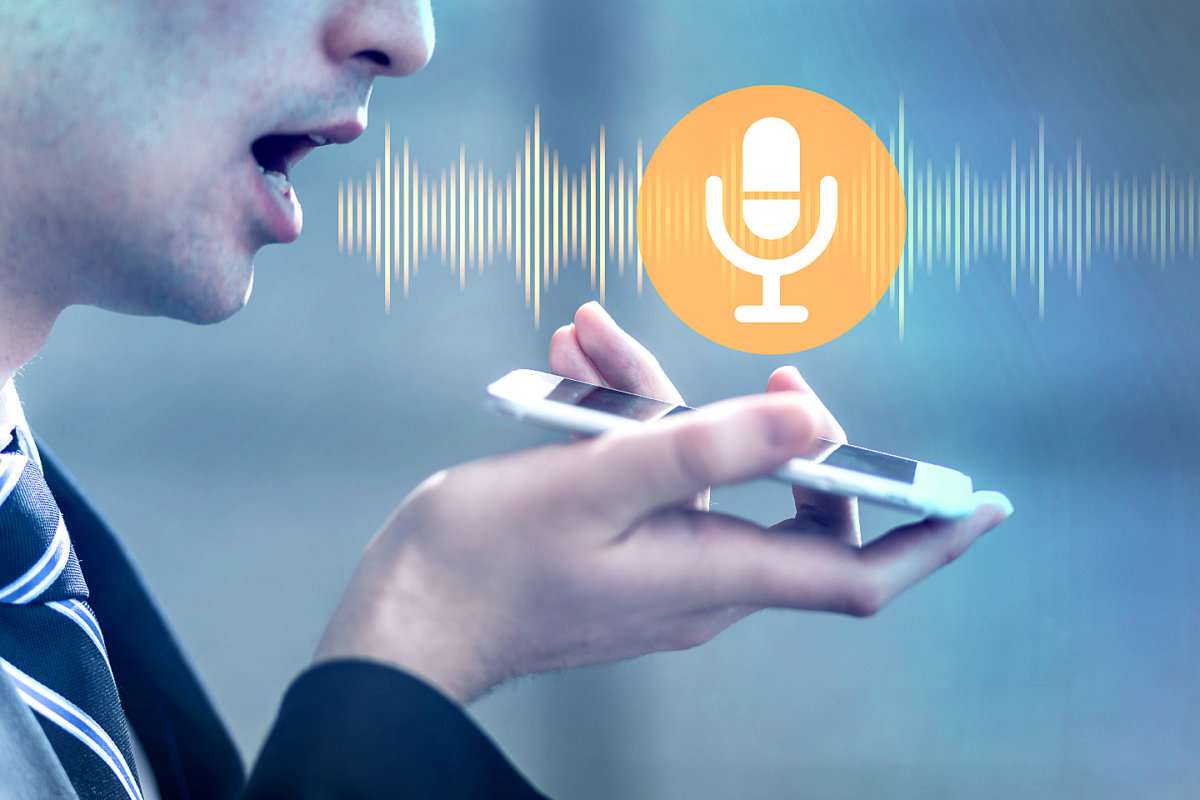
\includegraphics[width=0.9\textwidth]{figs/voice.jpg}%
	
}

\frame{
	\frametitle{ Search engines   }
	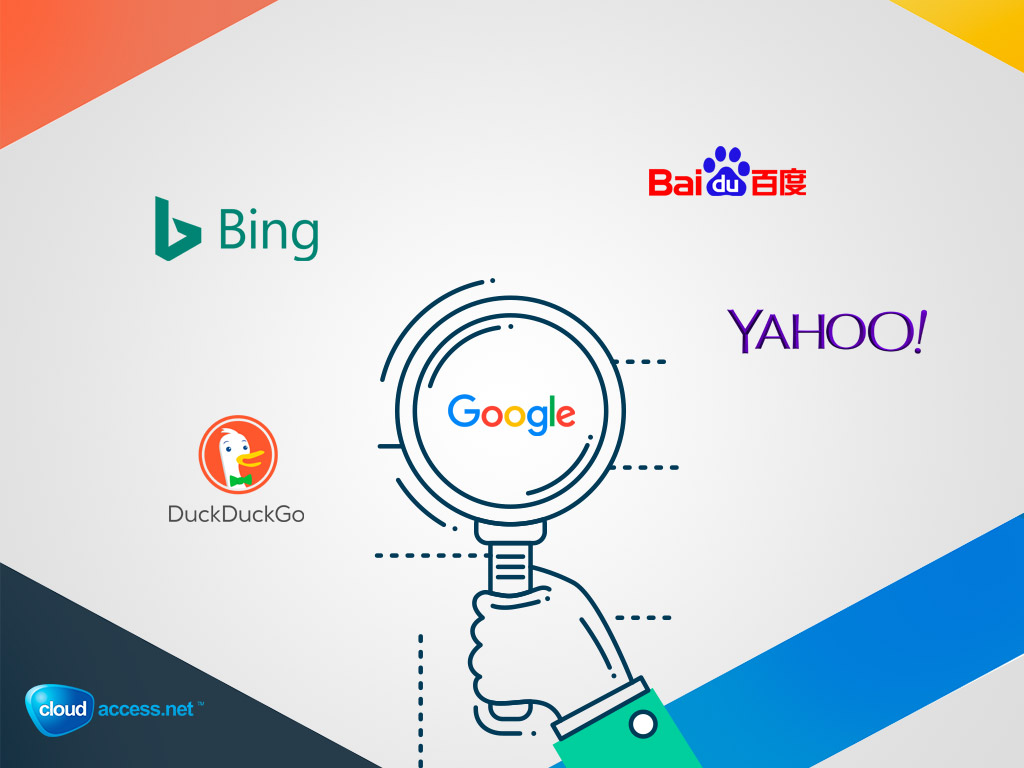
\includegraphics[width=1\textwidth]{figs/s.jpg}%
	  
}

\frame{
	\frametitle{ Coputer vision    }
	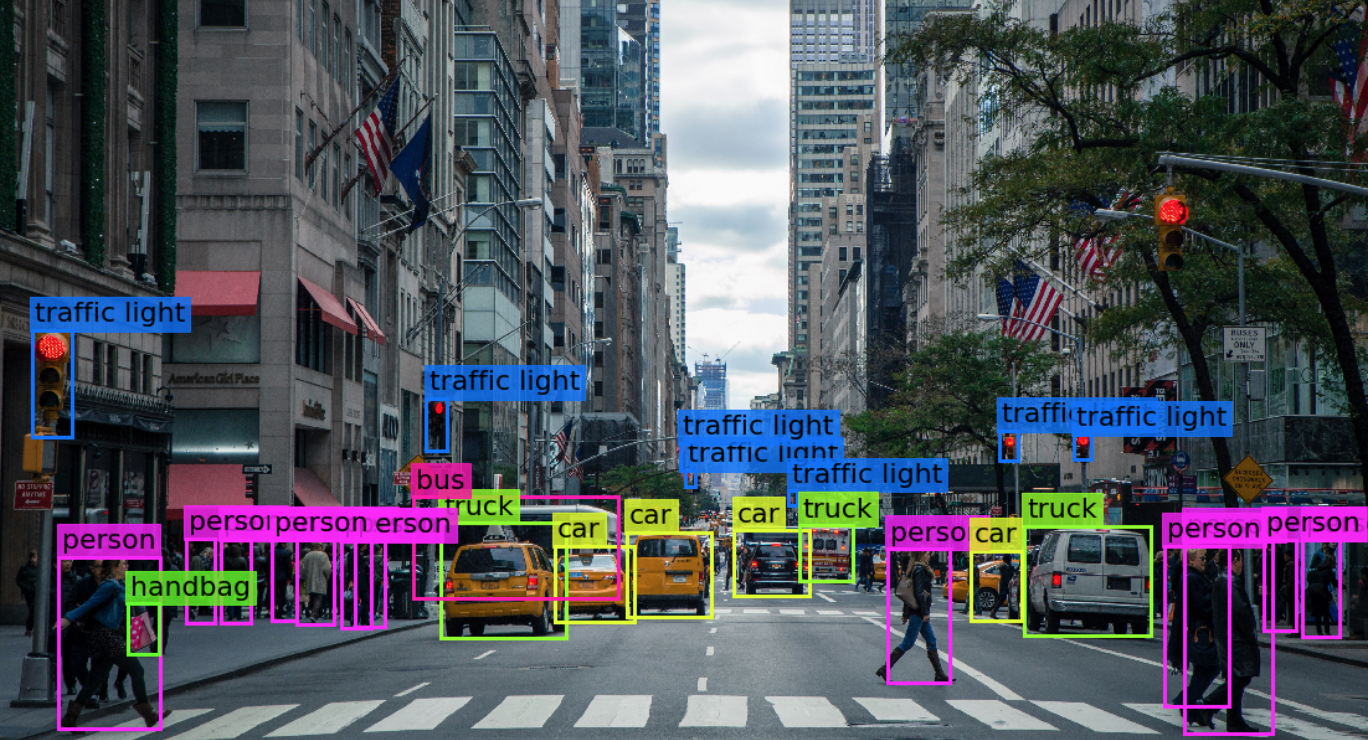
\includegraphics[width=1\textwidth]{figs/cv.png}%
	
}
\frame{
	\frametitle{ Everywhere ...    }
If you have enogh data, You surely can apply machine learning to it 
	
}
\section{Learning types}
\logo{}
\frame{
 
  	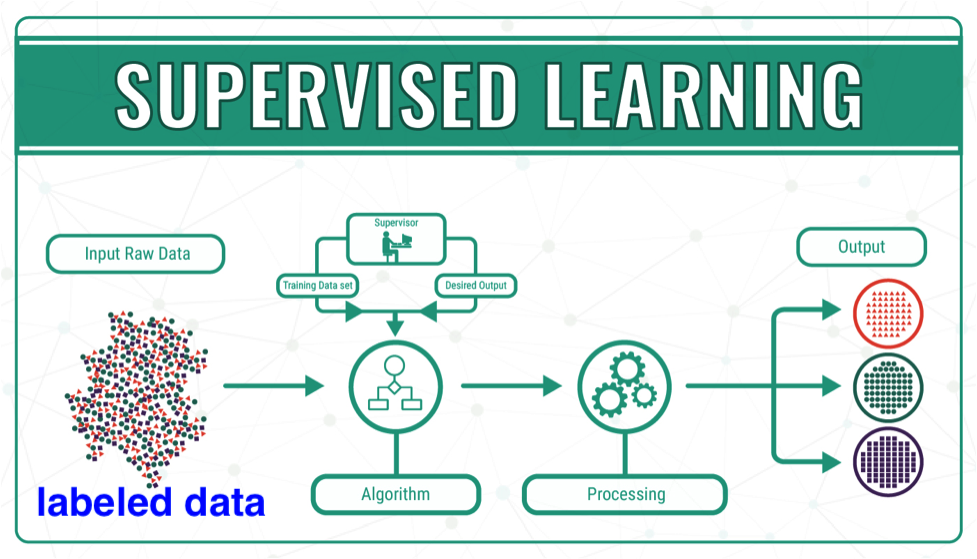
\includegraphics[width=1\textwidth]{figs/sup.png}%
}
\frame{
	
	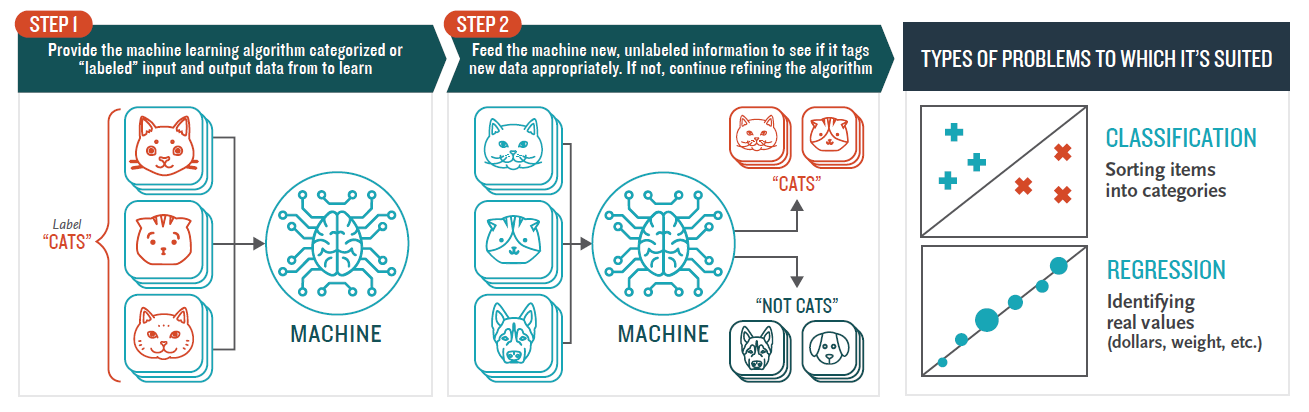
\includegraphics[width=1.\textwidth,height=5cm]{figs/sup2.png}%
}
\frame{
	\frametitle{ Regression  }
Regression is a technique from statistics that is used to predict values of a desired target \textbf{quantity} when the target quantity is \textbf{continuous}
	
}
\frame{
	\frametitle{Regression}
	\center
	\pgfdeclareimage[height=6cm]{CDCS}{figs/regression.jpg}
	\pgfuseimage{CDCS}
}
\frame{
	\frametitle{Regression}
	\center
	\pgfdeclareimage[height=6cm]{CDCS}{figs/house.jpg}
	\pgfuseimage{CDCS}
}

\frame{
		\frametitle{Classification}
Classification is the process of predicting \textbf{the class} of given data points. Classes are sometimes called as \textbf{targets/ labels or categories}. Classification predictive modeling is the task of approximating a mapping function (f) from input variables (X) to \textbf{discrete output} variables (y).


}

\frame{
	\frametitle{Classification examples}
	\center
	\pgfdeclareimage[height=5cm]{CDCS}{figs/teext.png}
	\pgfuseimage{CDCS}
}




\logo{}
\frame{
		\frametitle{Unsupervised learning}
	Unsupervised Learning is a class of Machine Learning techniques to find the patterns in data. The data given to unsupervised algorithm are \textbf{not labelled}, which means only the input variables(X) are given with no corresponding output variables.

}
\frame{
	\frametitle{Unsupervised learning}
	Unsupervised Learning is a class of Machine Learning techniques to find the patterns in data. The data given to unsupervised algorithm are \textbf{not labelled}, which means only the input variables(X) are given with no corresponding output variables.\\
	
	
		Given an \textbf{Unlabled data} to an algorithm , this algorithm tries to find if there are \textbf{groups, clusters} within the given data.
}


\frame{
	\frametitle{Unsupervised learning}
	\center
	\pgfdeclareimage[height=5.5cm]{CDCS}{figs/non.jpg}
	\pgfuseimage{CDCS}
}
\frame{
	\frametitle{Clustering }
Clustering is a Machine Learning technique that involves the \textbf{grouping} of data points. Given a set of \textbf{unlabled data}, we can use a clustering algorithm to \textbf{group} each data point into a \textbf{specific group}. In theory, data points that are in the \textbf{same} group should have \textbf{similar properties and/or features}, while data points in \textbf{different} groups should have \textbf{highly dissimilar properties and/or features}
	
}

\frame{
		\frametitle{Association rules }
Association rule mining is the data \textbf{mining} process of \textbf{finding the rules} that may govern associations and causal objects between sets of items. So in a given transaction with multiple items, it tries to find the rules that govern\textbf{ how or why such items} are often \textbf{bought together}.

}
\frame{
	\frametitle{Association rules mining}
	\center
	\pgfdeclareimage[width=\linewidth]{mark}{figs/mark.jpg}
	\pgfuseimage{mark}
}

\frame{
	\frametitle{Unsupervised learning Vs. Supervised learning}
	\center
	\pgfdeclareimage[height=5.7cm]{CDCS}{figs/vs.png}
	\pgfuseimage{CDCS}
}


\frame{
	\frametitle{Where to start ML ? }

\begin{itemize}
	\item Basics are essential 
		\item Theorical background is essential in ML , use frameworks for practice 
		\item Step by step  
	\item Statistics and interpretations  
		\item Love what you are doing  
\end{itemize}
}
\frame{
	AI Pionneers are alive !
	\frametitle{Usefull ressources}
	\center
	\pgfdeclareimage[height=5.7cm,width=\linewidth]{CDCS}{figs/ai.jpg}
	\pgfuseimage{CDCS}
}
\frame{

	\frametitle{Usefull ressources}
	
	\begin{itemize}
		\item Machine learning course at corsera, full course about Machine learning, provided by Andrew NJ - Professor at Stanford University and AI cheig at Baidu. 
		\item MIT opencourseware
		\item Medium and Towards Data science Blogs 
		\item Google things .. 
	\end{itemize}
}
\frame{
	
	\frametitle{Advanced ML applications}
}
\frame{
 
	\center
	\pgfdeclareimage[width=\linewidth,height=6.7cm]{CDCS}{figs/qst.jpg}
	\pgfuseimage{CDCS}
}


\section{Machine learning concepts}
\logo{}
\frame{
    \frametitle{Data split}

}

\frame{
	\frametitle{Overfitting and underfitting}
	
}

\frame{
	\frametitle{Cross validation }
	
}

\frame{
	\frametitle{Boosting}
	
}

 

\section{Advanced ML applications}
\logo{\pgfuseimage{inf}}
\frame{
	\frametitle{Ambiente de experimentação}
	
	\begin{itemize}
		\item \textit{Hardware}: 2 CPU AMD@1.7Ghz, 12 cores/CPU e 47GB RAM.
		\item \textit{Software}: Ubuntu x64 12.04, Hadoop 2.2.0, Sun JDK 1.7.
	\end{itemize}
}

\logo{\pgfuseimage{inf}}
\frame{
	\frametitle{Configuração dos experimentos}
	Texto texto texto texto texto texto texto texto
	\begin{table}
		\renewcommand{\figurename}{Table}
		\centering
		\begin{tabular}{|l|c|c|}
			\hline 
			  & Coluna1 & Coluna2 \\ 
			\hline 
			\textit{Linha1} & 1 & 2 \\ 
			\hline 
			\textit{Linha2} Vcores & 3 & 4 \\ 
			\hline 
		\end{tabular}
	\end{table}
}


\logo{}
\frame{
	\frametitle{Resultados de desempenho}
	
	\pgfdeclareimage[height=6cm]{totalVcores}{figs/Figura12-totalCores.png}
    %TODO fig colectInt
    \pgfuseimage{totalVcores}
}



\section{ Ressrouces }
\logo{\pgfuseimage{inf}}
\frame{
   \frametitle{Conclusão}
   	\begin{itemize}
   		\item Item
        \item Item
        \item Item
   	\end{itemize}
}

\logo{\pgfuseimage{inf}}
\frame{
   \frametitle{Trabalhos Futuros}
   	\begin{itemize}
   		\item Item
        \item Item
        \item Item
   	\end{itemize}
}


\section{Questions}
\logo{}
\frame{
    \frametitle{Referências}
    \begin{itemize}
	\begin{tiny}
    	   \item DEY, A. K. Understanding and Using Context. Personal Ubiquitous Comput., London, UK, UK, v.5, n.1, p.4-7, Jan. 2001.
       \item MAAMAR, Z.; BENSLIMANE, D.; NARENDRA, N. C. What can context do for web services? Commun. ACM, New York, NY, USA, v.49, n.12, p.98-103, Dec. 2006.
       \item KUMAR, K. A. et al. CASH: context aware scheduler for hadoop. In: INTERNATIONAL CONFERENCE ON ADVANCES IN COMPUTING, COMMUNICATIONS AND INFORMATICS, New York, NY, USA. Proceedings. . . ACM, 2012. p.52-61. (ICACCI '12).
       \item ZAHARIA, M. et al. Improving MapReduce performance in heterogeneous environments. In: USENIX CONFERENCE ON OPERATING SYSTEMS DESIGN AND IMPLEMENTATION, 8., Berkeley, CA, USA. Proceedings. . . USENIX Association, 2008. p.29-42. (OSDI'08).
       \item TIAN, C. et al. A Dynamic MapReduce Scheduler for Heterogeneous Workloads. In: EIGHTH INTERNATIONAL CONFERENCE ON GRID AND COOPERATIVE COMPUTING, 2009., Washington, DC, USA. Proceedings. . . IEEE Computer Society, 2009. p.218-224. (GCC '09).
        \item CHEN, Q. et al. SAMR: a self-adaptive mapreduce scheduling algorithm in heterogeneous environment. In: IEEE INTERNATIONAL CONFERENCE ON COMPUTER AND INFORMATION TECHNOLOGY, 2010., Washington, DC, USA. Proceedings. . . IEEE Computer Society, 2010. p.2736-2743. (CIT '10).

	\end{tiny}
    \end{itemize}
}

\logo{}
\frame{
    \frametitle{Referências (Continuação)}
    \begin{itemize}
    \begin{tiny}
       \item RASOOLI, A.; DOWN, D. G. Coshh: a classification and optimization based scheduler for heterogeneous hadoop systems. In: SC COMPANION: HIGH PERFORMANCE COMPUTING, NETWORKING STORAGE AND ANALYSIS, 2012., Washington, DC, USA. Proceedings. . . IEEE Computer Society, 2012. p.1284-1291. (SCC '12).
       \item ISARD, M. et al. Quincy: fair scheduling for distributed computing clusters. In: ACM SIGOPS 22ND SYMPOSIUM ON OPERATING SYSTEMS PRINCIPLES, New York, NY, USA. Proceedings. . . ACM, 2009. p.261-276. (SOSP '09).
       \item XIE, J. et al. Improving MapReduce performance through data placement in heterogeneous Hadoop clusters. In: PARALLEL AND DISTRIBUTED PROCESSING, WORKSHOPS AND PHD FORUM (IPDPSW). Anais. . . IEEE International Symposium, 2010.
       \item HADOOP, A. Arquitetura do HDFS. http://hadoop.apache.org/docs/current/hadoop-project-dist/hadoop-hdfs/Federation.html, Acesso em novembro de 2013.
       \item HADOOP, A. Arquitetura do YARN. http://hadoop.apache.org/docs/current/hadoop-yarn/hadoop-yarn-site/YARN.html, Acesso em novembro de 2013.

	\end{tiny}
    \end{itemize}
}





\begin{frame}
\titlepage
\end{frame}

\end{document}